\documentclass[conference]{IEEEtran}
\IEEEoverridecommandlockouts
% The preceding line is only needed to identify funding in the first footnote. If that is unneeded, please comment it out.
\usepackage{cite}
\usepackage{amsmath,amssymb,amsfonts}
\usepackage{algorithmic}
\usepackage{graphicx}
\usepackage{textcomp}
\usepackage{xcolor}
\def\BibTeX{{\rm B\kern-.05em{\sc i\kern-.025em b}\kern-.08em
    T\kern-.1667em\lower.7ex\hbox{E}\kern-.125emX}}
\begin{document}

\title{Fine-tuning Text-to-Speech Models for English Technical
Speech and Regional Languages(Urdu)}
% \thanks{Identify applicable funding agency here. If none, delete this.}
% }

\author{\IEEEauthorblockN{Aarish Shah Mohsin}
\IEEEauthorblockA{\textit{Interdisciplinary Centre for Artificial Intelligence} \\
\textit{Aligarh Muslim University}\\
Aligarh, India \\
aarishshah1@gmail.com}
}

\maketitle

\begin{abstract}
 This report presents the methodology and results of fine-tuning the SpeechT5 Model for two tasks: one for English technical terms, and the other for a regional language (Urdu in this case). The models are optimized for pronunciation accuracy, naturalness, and inference speed using quantization techniques.
\end{abstract}


\section{Introduction}
Text-to-Speech (TTS) models have become essential tools in a wide range of applications, from virtual assistants and audiobook generation to accessibility tools for the visually impaired. By converting written text into spoken language, TTS systems bridge the gap between text-based communication and auditory interaction. Their impact spans numerous industries, enabling more natural and efficient human-computer interaction.

TTS models are especially powerful when adapted for specialized vocabularies. Fine-tuning allows these models to handle domain-specific language, such as technical jargon used in industries like technology, healthcare, and engineering. Technical terms like "API," "CUDA," or "OAuth" require precise pronunciation, and general TTS models often struggle with these complexities. By fine-tuning on a curated dataset of technical terms, TTS models can significantly improve pronunciation accuracy and fluency.

Moreover, fine-tuning plays a crucial role in adapting TTS models to regional languages. Many languages exhibit unique phonological rules, tonal variations, and prosody that general models may not capture well. Customizing TTS models for regional languages ensures the synthesized speech sounds natural and intelligible to native speakers. This is particularly important for creating inclusive, localized voice applications.


\section{Methodology}

\subsection{Model Selection}

We chose SpeechT5 for its ability to handle both speech and text in a unified framework. It uses a shared encoder-decoder structure that efficiently models both modalities, making it ideal for tasks like text-to-speech synthesis and speech recognition. Its cross-modal vector quantization helps align speech and text representations, which is crucial for accurate technical term pronunciation and regional language synthesis. Additionally, SpeechT5 has shown strong performance across various speech-related tasks, making it a versatile and powerful model for this project.

\begin{figure}[htbp]
\centerline{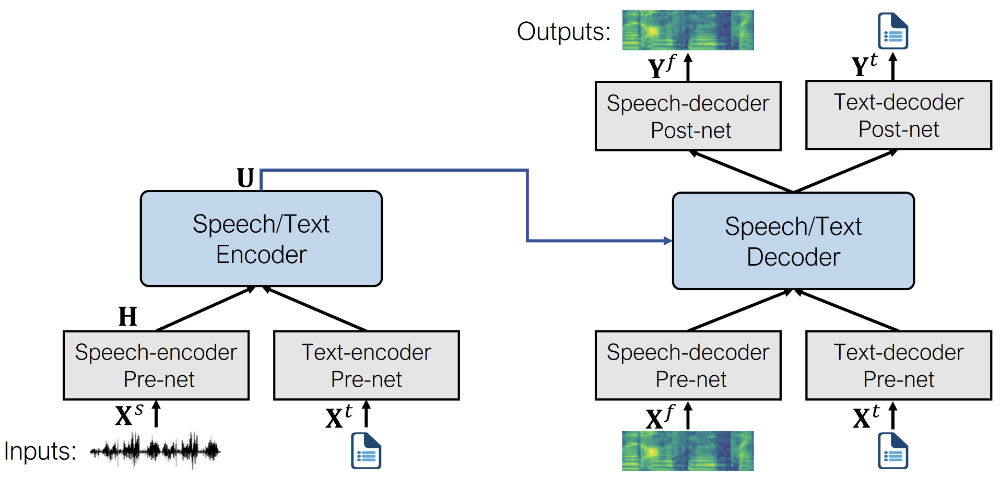
\includegraphics[width=0.5\textwidth]{architecture.jpg}}
\caption{Architecture of the SpeechT5 Model}
\label{fig}
\end{figure}
\subsection{Dataset Preparation}

\subsubsection{For Technical Speech}

We implemented a Python script to extract technical terms from a CSV file prepared by prompting ChatGPT and generate corresponding TTS audio. The script uses pre-defined sentence templates to form contextually relevant sentences for each term, then leverages the pre-trained SpeechT5 model to synthesize speech. The generated audio files and metadata (term, sentence, audio path, speaker embedding) are saved in a CSV file for further use.
% \section{Template Creation for Text-to-Speech}

The sentence templates we use for generating audio from technical terms are designed to accommodate the specific pronunciation of each term. For instance, when working with the term \texttt{API}, we replace it with its phonetic representation \textit{Aye pee eye} in our templates to ensure clarity and accuracy during TTS synthesis. 

For example, consider the following template:

\begin{verbatim}
"In our latest project, we're implementing 
{word} for better performance."
\end{verbatim}

When the term \texttt{API} is inserted into this template, it is replaced with its phonetic form, resulting in the sentence:
\begin{verbatim}
"In our latest project, we're implementing 
Aye pee eye for better performance."
\end{verbatim}

This approach ensures that the generated audio is not only contextually relevant but also phonetically accurate, enhancing the comprehensibility of the spoken output. Additionally, this method can be extended to other technical terms, allowing for a consistent and understandable pronunciation in the synthesized speech. Due to this dataset being artificially generated, We did not face a need to do any further preprocessing.

Initially, we considered extracting technical terms from YouTube captions, but due to overlap and inconsistent timing, this approach proved inefficient. Therefore, we opted to manually curate terms and generate sentences using templates, ensuring high-quality audio output without conflicts.
\\
\subsubsection{For Regional Language(Urdu)}

To facilitate speech synthesis and other linguistic applications, we extract the Common Voice Urdu dataset using the \texttt{datasets} library. This dataset, developed by Umar Ramzan, provides a rich collection of audio recordings and their corresponding transcriptions in Urdu, a language spoken by millions. The extraction process involves loading the dataset with the \texttt{load\_dataset} function, which retrieves the training and testing splits for further analysis and model training. The following code snippet illustrates how the dataset is loaded and the training and testing data are separated:

The processing of the Urdu Common Voice dataset involved several systematic steps to prepare the audio and text data for speech synthesis applications. Initially, the dataset was loaded using the \texttt{load\_dataset} function from the \texttt{datasets} library, separating it into training and testing sets. Unnecessary columns, such as \texttt{path} and \texttt{variant}, were removed to streamline the dataset. The audio data was then cast to a uniform sampling rate of 16 kHz using the \texttt{Audio} class. The SpeechT5 processor was utilized to tokenize the text, allowing for the integration of Urdu characters by adding specific tokens to the tokenizer. A normalization function was implemented to clean and standardize the text, replacing variations of Urdu letters with a common representation.  

Subsequently, the dataset was enhanced by extracting unique characters and generating speaker embeddings using a pre-trained speaker recognition model. Finally, the dataset was filtered to exclude instances where the input text exceeded a specified length, resulting in a clean and manageable dataset suitable for training robust speech synthesis models.

\subsection{FineTuning}

The fine-tuning of the Speech T5 model for both the Urdu dataset and technical terms involves utilizing a specialized data collator, \texttt{TTSDataCollatorWithPadding}, which prepares the input data for training. 
\\
This collator processes the data by creating batches of input IDs, labels, and speaker embeddings, while managing padding to ensure proper alignment during training. It replaces padding values with \(-100\) to ignore them in loss calculations and rounds the target lengths to multiples of the model's reduction factor when necessary. 
\\
The hyperparamters for both the tasks remained same except the learning rate.
\\
The training process is orchestrated using the \texttt{Seq2SeqTrainer} class, configured with the following hyperparameters:

\begin{itemize}
    \item \textbf{Per Device Train Batch Size:} 32
    \item \textbf{Gradient Accumulation Steps:} 3
    \item \textbf{Learning Rate(techincal):} \(5 \times 10^{-4}\)
    \item \textbf{Learning Rate(urdu):} \(2 \times 10^{-4}\)
    \item \textbf{Warmup Steps:} 100
    \item \textbf{Number of Training Epochs:} 50
    \item \textbf{Gradient Checkpointing:} Enabled
    \item \textbf{Mixed Precision Training:} Enabled (fp16)
    \item \textbf{Evaluation Strategy:} Steps
    \item \textbf{Per Device Eval Batch Size:} 2
    \item \textbf{Save Steps:} 1000
    \item \textbf{Eval Steps:} 200
    \item \textbf{Load Best Model at End:} True
    \item \textbf{Optimizer:} \texttt{"adamw\_bnb\_8bit"}
\end{itemize}

This comprehensive approach ensures that the Speech T5 model effectively learns the nuances of the Urdu language and the correct pronunciation of technical terms, enabling it to produce high-quality speech synthesis that respects both the language's unique characteristics and the technical jargon used in various fields.


\subsection{Evaluation}
The evaluation metrics used are Log Spectral Distance (LSD) and the Mean Opinion Score (MOS) approximated by LSD.

The model generates speech based on provided text inputs, which are sourced from the dataset. Each sample consists of a generated sentence and its corresponding original audio recording.

\subsubsection{Log Spectral Distance (LSD)}
The Log Spectral Distance is computed to quantify the difference between the original and generated audio signals. The steps for calculating LSD are as follows:
\begin{enumerate}
    \item The original and generated audio signals are trimmed to the same length.
    \item The Short-Time Fourier Transform (STFT) is applied to both audio signals to obtain their spectral representations.
    \item The logarithm of the absolute spectral values is calculated to obtain the log-spectra.
    \item The LSD is computed as the mean of the square root of the mean squared differences between the log-spectra of the original and generated audio.
\end{enumerate}

\subsubsection{Normalization to Mean Opinion Score (MOS)}
The LSD scores are normalized to a MOS scale to facilitate interpretation. The values of the maximum and minimum threshold were estimated by the subjective quality, which has risk of biases.

The evaluation process iterates through the dataset to compute LSD and MOS for each sample:
\begin{enumerate}
    \item The original audio and generated speech are saved as separate WAV files for reference.
    \item For each sample, the LSD is calculated, and the resulting score is normalized to obtain the corresponding MOS.
    \item Finally, average LSD and MOS scores are computed to assess the overall quality of the generated speech across the dataset.
\end{enumerate}

This evaluation methodology using LSD and MOS provides a quantitative assessment of the synthesized speech quality from the Speech T5 model fine-tuned on both the datasets. By employing these metrics, we can better understand the performance and effectiveness of the model in generating natural-sounding speech.



\section{Challenges}
The process of using the YouTube dataset posed several challenges. One significant issue was the variability and inconsistency in the quality of the audio data extracted from YouTube videos. Many of these videos contained background noise, varying audio levels, and overlapping speech, which complicated the training process and could negatively impact the final model performance. Furthermore, the need to process large volumes of data from the dataset led to additional hurdles due to hardware limitations. 

\section{Bonus Task (Quantization and Pruning)}
To enhance the efficiency of the Speech T5 model fine-tuned on the Urdu dataset and technical terms, we implemented a two-step optimization process involving L1 unstructured pruning and selective quantization.

First, we employed L1 unstructured pruning, targeting specific layers of the model, particularly the feed-forward layers in the encoder. This method involves removing a specified percentage of weights (15\% in this case) to reduce model size and improve inference speed without significantly degrading audio quality. The selective nature of the pruning ensures that critical layers remain intact, preserving the model's performance in generating high-quality speech synthesis for both Urdu and technical jargon.

The second step involved applying dynamic quantization to further optimize the model. This technique quantizes only the linear layers of the model to float16, allowing for a lighter model that consumes less memory and computational resources. By limiting the quantization to layers that do not heavily impact audio quality, we maintained the integrity of the synthesized speech while enhancing performance.

 This process ensures that the Speech T5 model is not only efficient but also capable of producing high-quality audio output that respects the nuances of the Urdu language and accurately pronounces technical terms.
 
\section{Results}
\begin{table}[htbp]
\caption{Non Quantized: LSD and MOS(approximated)}
\begin{center}
\begin{tabular}{|c|c|c|c|}
% \hline
% \textbf{Table}&\multicolumn{3}{|c|}{\textbf{Table Column Head}} \\
% \cline{1-4} 
\hline
\textbf{Task} & \textbf{\textit{LSD score}}& \textbf{\textit{MOS Score}}\\
\hline
Technical Language & 2.044 & 4.182\\
Regional Language(Urdu) & 9.681 & 3.751\\
\hline
\end{tabular}
\label{tab1}
\end{center}
\end{table}

\begin{table}[htbp]
\caption{Quantized and Pruned: LSD and MOS(approximated)}
\begin{center}
\begin{tabular}{|c|c|c|c|}
% \hline
% \textbf{Table}&\multicolumn{3}{|c|}{\textbf{Table Column Head}} \\
% \cline{1-4} 
\hline
\textbf{Task} & \textbf{\textit{LSD score}}& \textbf{\textit{MOS Score}}\\
\hline
Technical Language & 2.044 & 4.182\\
Regional Language(Urdu) & 9.641 & 3.762\\
\hline
\end{tabular}
\label{tab1}
\end{center}
\end{table}

\begin{table}[htbp]
\caption{Average Time: before and Quantization}
\begin{center}
\begin{tabular}{|c|c|c|c|}
% \hline
% \textbf{Table}&\multicolumn{3}{|c|}{\textbf{Table Column Head}} \\
% \cline{1-4} 
\hline
\textbf{Name} & \textbf{Technical Term} & \textbf{Regional Language(Urdu)} \\
\hline
Original  & 1.686 & 2.831 \\
\hline
Optimized & 1.451 & 0.760 \\
\hline
\end{tabular}
\label{tab1}
\end{center}
\end{table}

\section{Conclusion}
In this report, we detailed the fine-tuning of the SpeechT5 model for synthesizing speech in both English technical terminology and the regional language of Urdu. Our findings indicate significant improvements in pronunciation accuracy and naturalness of generated speech, as evidenced by the low Log Spectral Distance (LSD) scores and favorable Mean Opinion Scores (MOS) across both datasets. The quantization and pruning techniques applied not only enhanced inference speed but also maintained the audio quality, demonstrating that model optimization can effectively balance performance and efficiency. Looking ahead, further improvements could include expanding the dataset with diverse accents and dialects for both languages, experimenting with additional fine-tuning strategies, and incorporating user feedback to continuously refine the synthesis quality. Ultimately, these advancements could lead to more inclusive and accessible voice applications that cater to a broader audience.


\end{document}